% Figure 1 of "The architecture of blockchain value: capabilities, pillars, and growth dynamics"
% (Papadogiannis, 2026, Front. Blockchain 9:1747512). Drawing code as in the author's manuscript.
% Compile with: pdflatex fig1_transaction_flow.tex
\documentclass[border=6pt]{standalone}
\usepackage{amsmath, amssymb}
\usepackage{tikz}
\usetikzlibrary{positioning, shapes, arrows.meta, calc, backgrounds}
\begin{document}
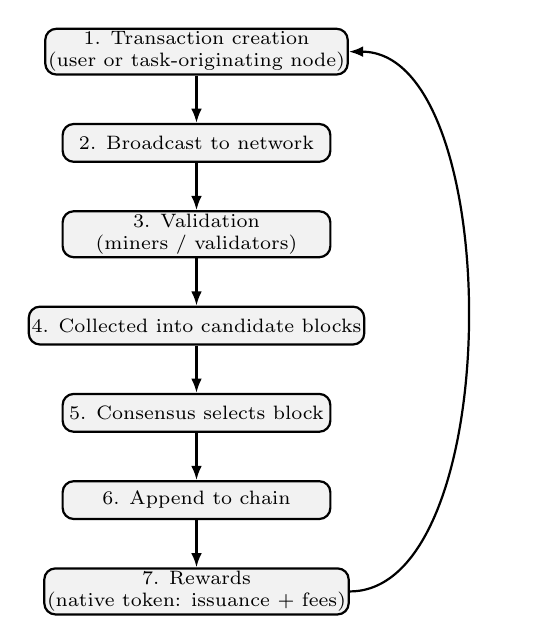
\begin{tikzpicture}[
  font=\scriptsize,
  node distance=0.6cm,
  box/.style={rounded corners, draw=black, thick, fill=gray!10, inner sep=1pt, align=center, minimum width=3.4cm, minimum height=0.48cm},
  arrow/.style={-{Latex[length=1.8mm]}, thick}
]
\node[box] (create)   {1. Transaction creation \\ \scriptsize(user or task-originating node)};
\node[box, below=of create]   (broadcast) {2. Broadcast to network};
\node[box, below=of broadcast] (validate) {3. Validation \\ \scriptsize(miners / validators)};
\node[box, below=of validate]  (group)    {4. Collected into candidate blocks};
\node[box, below=of group]     (cons)     {5. Consensus selects block};
\node[box, below=of cons]      (append)   {6. Append to chain};
\node[box, below=of append]    (reward)   {7. Rewards \\ \scriptsize(native token: issuance + fees)};

\draw[arrow] (create) -- (broadcast);
\draw[arrow] (broadcast) -- (validate);
\draw[arrow] (validate) -- (group);
\draw[arrow] (group) -- (cons);
\draw[arrow] (cons) -- (append);
\draw[arrow] (append) -- (reward);
\draw[arrow] (reward.east) .. controls +(2,0) and +(2,0) .. (create.east);
\end{tikzpicture}
\end{document}
